\documentclass[12pt,a4paper]{article}
\usepackage[T1]{fontenc}
\usepackage[utf8]{inputenc}
\usepackage{lmodern}
\usepackage[brazil]{babel}
\usepackage{amsmath,amssymb}
\usepackage{graphicx}
\usepackage{float}
\usepackage{indentfirst}
\usepackage{booktabs}
\usepackage[margin=2.5cm]{geometry}
\usepackage{listings}
\usepackage{xcolor}

\graphicspath{{figs/}}

% ----- estilo das listagens de codigo (MATLAB) -----
\definecolor{azulkw}{rgb}{0.10,0.10,0.85}
\definecolor{verdecmt}{rgb}{0.0,0.5,0.0}
\definecolor{vermstr}{rgb}{0.70,0.0,0.0}
\lstdefinestyle{matlab}{
  language=Matlab,
  numbers=left,
  numberstyle=\tiny\color{gray},
  frame=single,
  rulecolor=\color{black!55},
  basicstyle=\ttfamily\small,
  keywordstyle=\color{azulkw},
  commentstyle=\color{verdecmt},
  stringstyle=\color{vermstr},
  showstringspaces=false,
  breaklines=true,
  columns=fullflexible,
  tabsize=2,
  captionpos=b,
  aboveskip=1.2em,
  belowskip=1.2em,
}
\lstset{style=matlab}

\setlength{\parskip}{0.4em}

\begin{document}

% ==================== CAPA ====================
\begin{titlepage}
\centering
{\large\bfseries UNIVERSIDADE TECNOL\'OGICA FEDERAL DO PARAN\'A\par}
{\large\bfseries CURSO DE ENGENHARIA DE COMPUTA\c{C}\~AO\par}
\vspace{0.4cm}
{\normalsize ELEQ30 - An\'alise de Sistemas Lineares\par}
{\normalsize Professor C\'esar Janeczko\par}

\vspace{3.2cm}
{\LARGE\bfseries Relat\'orio: Pr\'atica 4\par}
\vspace{0.4cm}
{\large\bfseries Filtros Window-sinc (FIR) / Imagem H\'ibrida\par}

\vspace{1.6cm}
{\large\bfseries Disciplina: An\'alise de Sistemas Lineares\par}

\vspace{2.8cm}
{\large Leonardo Pereira Shibata\par}
\vspace{0.2cm}
{\large Sergio Roncato Maccari\par}

\vfill
{\large Curitiba, Junho de 2026\par}
\end{titlepage}

% ==================== QUESTAO 1 ====================
\section*{Quest\~ao 1: Filtro Window-sinc passa-baixas (FWSPB)}

A rotina em \textsc{Basic} fornecida no enunciado foi convertida para uma fun\c{c}\~ao
em \textit{Matlab} que recebe a ordem do filtro $M$ e a frequ\^encia de corte normalizada
$FC$ (entre $0$ e $0{,}5$) e retorna o n\'ucleo do filtro $H$, com $M+1$ coeficientes.
O n\'ucleo \'e a fun\c{c}\~ao \textit{sinc} amostrada e deslocada para o centro
$n = M/2$, garantindo fase linear:
%
\begin{equation}
h[n] = \frac{\sin\!\big(2\pi\,FC\,(n - M/2)\big)}{n - M/2},
\qquad h[M/2] = 2\pi\,FC ,
\end{equation}
%
sendo o segundo caso o limite da express\~ao quando $n = M/2$ (para evitar a
indetermina\c{c}\~ao $0/0$).

Conforme indicado no enunciado, a janela de \textbf{Hamming} da linha 280 do programa
original ($0{,}54 - 0{,}46\cos(2\pi n/M)$) foi \textbf{substitu\'ida pela janela de
Blackman}:
%
\begin{equation}
w[n] = 0{,}42 - 0{,}5\cos\!\Big(\tfrac{2\pi n}{M}\Big) + 0{,}08\cos\!\Big(\tfrac{4\pi n}{M}\Big).
\end{equation}
%
Por fim, o n\'ucleo \'e normalizado pela soma de seus coeficientes
($H = H/\sum H$), o que assegura ganho unit\'ario em corrente cont\'inua (DC).

\begin{lstlisting}[caption={Fun\c{c}\~ao FWSPB -- passa-baixas com janela de Blackman.}]
function H = FWSPB(M, FC)
    % Filtro Window-sinc PASSA-BAIXAS com janela de Blackman
    %   M  -> ordem do filtro (resulta em M+1 coeficientes)
    %   FC -> frequencia de corte normalizada (0 a 0.5)
    H  = zeros(1, M+1);
    m2 = M/2;
    for i = 0:M
        if (i - m2) == 0
            H(i+1) = 2*pi*FC;                       % limite da sinc no centro
        else
            H(i+1) = sin(2*pi*FC*(i - m2)) / (i - m2);
        end
        % --- Janela de Blackman (substitui a de Hamming) ---
        w = 0.42 - 0.5*cos(2*pi*i/M) + 0.08*cos(4*pi*i/M);
        H(i+1) = H(i+1) * w;
    end
    H = H / sum(H);                                 % ganho unitario em DC
end
\end{lstlisting}

% ==================== QUESTAO 2 ====================
\section*{Quest\~ao 2: Resposta em frequ\^encia do filtro passa-baixas}

\subsection*{2.a) Filtro com janela de Blackman ($FC = 0{,}15$ e $M = 100$)}

Com $FC = 0{,}15$ e $M = 100$ obt\^em-se um n\'ucleo de $101$ pontos. A
Figura~\ref{fig:2a_t} mostra a resposta ao impulso $h[n]$: trata-se de uma
\textit{sinc} sim\'etrica em torno de $n = M/2 = 50$ e suavizada nas extremidades
pela janela. A resposta em frequ\^encia (Figura~\ref{fig:2a_f}) \'e apresentada em
ganho linear e em atenua\c{c}\~ao (dB) -- em gr\'aficos separados dos do dom\'inio
do tempo, conforme solicitado.

\begin{figure}[H]
\centering
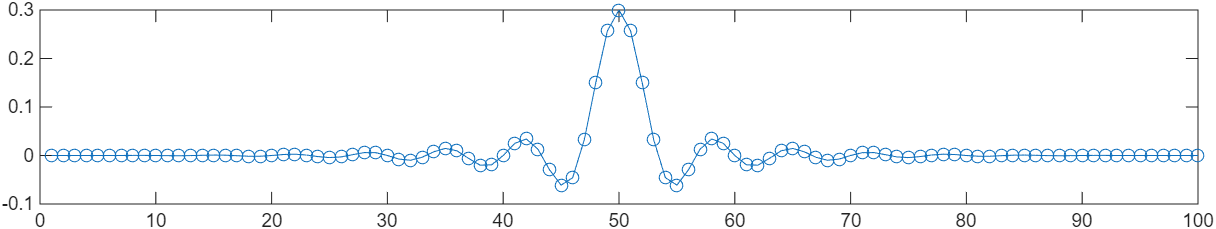
\includegraphics[width=0.82\textwidth]{fig_2a_tempo.png}
\caption{Resposta ao impulso $h[n]$ do FPB com janela de Blackman ($FC=0{,}15$, $M=100$).}
\label{fig:2a_t}
\end{figure}

\begin{figure}[H]
\centering
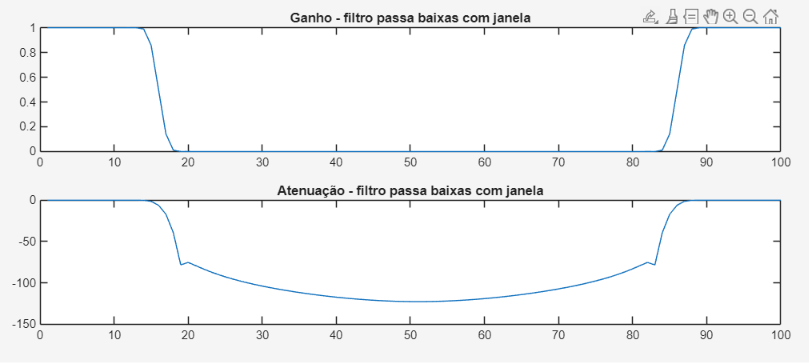
\includegraphics[width=0.82\textwidth]{fig_2a_freq.png}
\caption{Resposta em frequ\^encia do FPB com janela de Blackman: ganho (linear) e
atenua\c{c}\~ao (dB). A linha tracejada marca $FC = 0{,}15$.}
\label{fig:2a_f}
\end{figure}

O filtro apresenta banda de passagem plana (ganho~$\approx 1$) at\'e cerca de
$0{,}13$, transi\c{c}\~ao centrada em $FC = 0{,}15$ (ponto de meia amplitude,
$-6$~dB) e banda de rejei\c{c}\~ao com atenua\c{c}\~ao superior a $90$~dB. A
simetria de $h[n]$ em torno de $n=50$ confirma a fase linear do filtro.

\subsection*{2.b) Filtro sem a janela (janela retangular) -- \textit{ripple}}

Comentando-se o c\'alculo da janela (linha 280), o n\'ucleo passa a ser uma
\textit{sinc} simplesmente truncada, o que equivale a aplicar uma \textbf{janela
retangular}. A Figura~\ref{fig:2b_t} mostra que $h[n]$ termina abruptamente nas
bordas, e a Figura~\ref{fig:2b_f} revela o resultado disso no dom\'inio da
frequ\^encia.

\begin{lstlisting}[caption={Vers\~ao do FPB com a janela comentada (item 2.b).}]
function H = FWSPB_semjanela(M, FC)
    H  = zeros(1, M+1);
    m2 = M/2;
    for i = 0:M
        if (i - m2) == 0
            H(i+1) = 2*pi*FC;
        else
            H(i+1) = sin(2*pi*FC*(i - m2)) / (i - m2);
        end
        % w = 0.42 - 0.5*cos(2*pi*i/M) + 0.08*cos(4*pi*i/M);  % JANELA COMENTADA
        % H(i+1) = H(i+1) * w;
    end
    H = H / sum(H);
end
\end{lstlisting}

\begin{figure}[H]
\centering
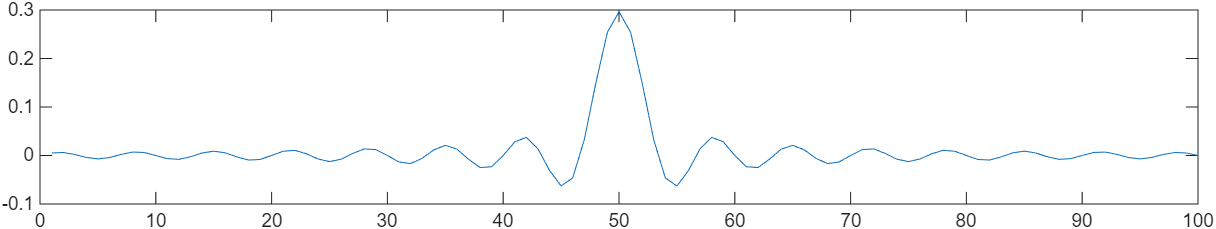
\includegraphics[width=0.82\textwidth]{fig_2b_tempo.png}
\caption{Resposta ao impulso $h[n]$ do FPB \textbf{sem} a janela (sinc truncada).}
\label{fig:2b_t}
\end{figure}

\begin{figure}[H]
\centering
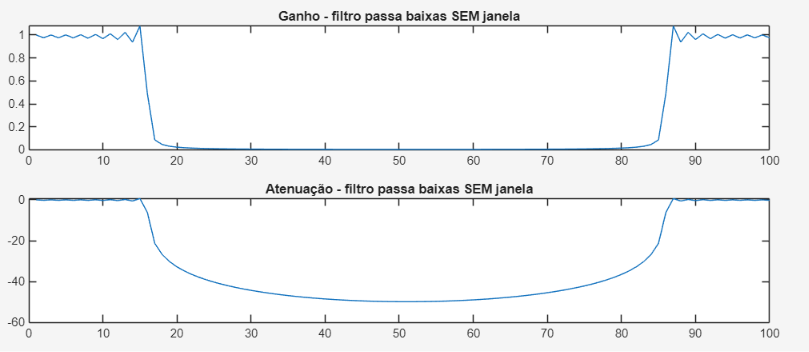
\includegraphics[width=0.82\textwidth]{fig_2b_freq.png}
\caption{Resposta em frequ\^encia do FPB sem a janela: observa-se \textit{ripple} na
banda de passagem e lobos laterais elevados na banda de rejei\c{c}\~ao.}
\label{fig:2b_f}
\end{figure}

\textbf{Conclus\~oes:} a remo\c{c}\~ao da janela faz surgir o \textit{ripple} de
Gibbs. Na banda de passagem aparece uma ondula\c{c}\~ao de aproximadamente
$4\%$ (pico a pico) e, na banda de rejei\c{c}\~ao, os lobos laterais decaem muito
lentamente, limitando a atenua\c{c}\~ao a cerca de $-21$ a $-35$~dB. Comparando com o
item~2.a, a janela de Blackman praticamente \textbf{elimina o \textit{ripple}} e leva
a atenua\c{c}\~ao para abaixo de $-90$~dB. O pre\c{c}o pago \'e uma banda de
transi\c{c}\~ao um pouco mais larga -- o cl\'assico compromisso entre n\'itidez da
transi\c{c}\~ao (janela retangular) e qualidade da rejei\c{c}\~ao (janela de Blackman).

% ==================== QUESTAO 3 ====================
\section*{Quest\~ao 3: Transforma\c{c}\~ao passa-baixas $\rightarrow$ passa-altas (FWSPA)}

Recolocada a janela (item 2.a), o filtro passa-altas (FPA) \'e obtido por
\textbf{invers\~ao espectral} do passa-baixas. Como o FPB tem fase linear (n\'ucleo
sim\'etrico), basta inverter o sinal de todos os coeficientes e somar um impulso
unit\'ario no centro:
%
\begin{equation}
h_{\text{PA}}[n] = \delta[n - M/2] - h_{\text{PB}}[n].
\end{equation}
%
Em frequ\^encia isso equivale a $H_{\text{PA}}(f) = 1 - H_{\text{PB}}(f)$, ou seja,
tudo o que era rejeitado passa a ser transmitido e vice-versa, mantendo-se a mesma
frequ\^encia de corte.

\begin{lstlisting}[caption={Fun\c{c}\~ao FWSPA -- passa-altas por invers\~ao espectral.}]
function H = FWSPA(M, FC)
    % Filtro PASSA-ALTAS obtido por inversao espectral do passa-baixas
    H = FWSPB(M, FC);              % parte do passa-baixas (com janela)
    H = -H;                        % inverte o sinal de todos os coeficientes
    H(M/2 + 1) = H(M/2 + 1) + 1;   % soma o impulso unitario no centro
end
\end{lstlisting}

Aplicando $FC = 0{,}15$ e $M = 100$ ao filtro do item~2, obt\^em-se os
resultados das Figuras~\ref{fig:3_t} e~\ref{fig:3_f}.

\begin{figure}[H]
\centering
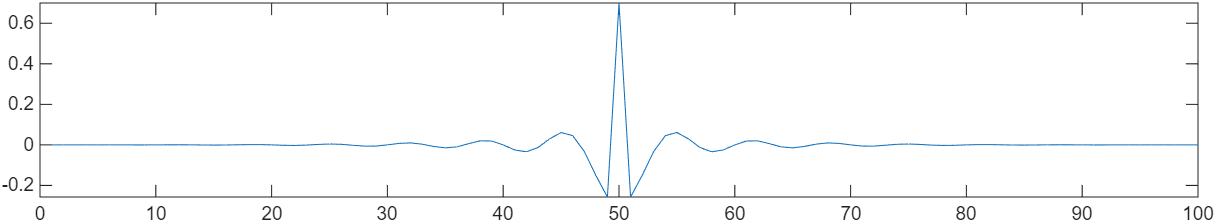
\includegraphics[width=0.82\textwidth]{fig_3_tempo.png}
\caption{Resposta ao impulso $h[n]$ do FPA ($FC=0{,}15$, $M=100$).}
\label{fig:3_t}
\end{figure}

\begin{figure}[H]
\centering
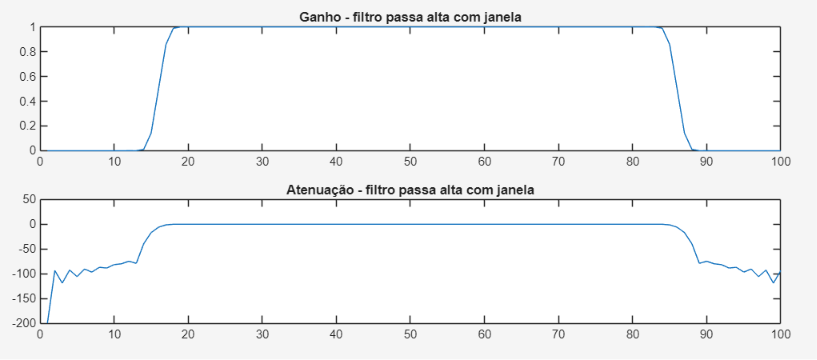
\includegraphics[width=0.82\textwidth]{fig_3_freq.png}
\caption{Resposta em frequ\^encia do FPA: ganho (linear) e atenua\c{c}\~ao (dB).}
\label{fig:3_f}
\end{figure}

A resposta \'e exatamente a imagem espelhada do passa-baixas: rejeita as
frequ\^encias abaixo de $0{,}15$ (atenua\c{c}\~ao $>90$~dB) e transmite as acima,
com ganho unit\'ario. No tempo, o n\'ucleo mant\'em a simetria (fase linear), agora
com o lobo central positivo cercado de lobos laterais negativos pr\'oximos.

% ==================== QUESTAO 4 ====================
\section*{Quest\~ao 4: Filtros passa-faixa e corta-faixa}

A partir dos filtros passa-baixas e passa-altas constru\'iram-se os filtros de
faixa, ambos com $100$ pontos ($101$ coeficientes), para as frequ\^encias de corte
inferior $0{,}15$ e superior $0{,}30$.

\textbf{Passa-faixa (FPF).} Para passar apenas a faixa entre $0{,}15$ e $0{,}30$,
coloca-se um passa-baixas com corte em $0{,}30$ \textbf{em cascata} com um
passa-altas com corte em $0{,}15$. No dom\'inio do tempo a cascata corresponde \`a
\textbf{convolu\c{c}\~ao} dos dois n\'ucleos (produto dos espectros). Usando
$M = 50$ em cada um, a convolu\c{c}\~ao resulta em $50+50+1 = 101$ coeficientes.

\textbf{Corta-faixa (FCF).} Para rejeitar a faixa entre $0{,}15$ e $0{,}30$,
somam-se (associa\c{c}\~ao \textbf{paralela}) um passa-baixas com corte em $0{,}15$
e um passa-altas com corte em $0{,}30$. Assim passam as frequ\^encias abaixo de
$0{,}15$ e acima de $0{,}30$, rejeitando-se a faixa central. Cada filtro tem
$M = 100$, e a soma mant\'em os $101$ coeficientes.

\begin{lstlisting}[caption={Constru\c{c}\~ao dos filtros passa-faixa e corta-faixa.}]
% ---- Passa-faixa (0.15 a 0.30): LP(0.30) em cascata com HP(0.15) ----
FPF = conv( FWSPB(50, 0.30), FWSPA(50, 0.15) );   % 101 coeficientes

% ---- Corta-faixa (0.15 a 0.30): LP(0.15) somado com HP(0.30) ----
FCF = FWSPB(100, 0.15) + FWSPA(100, 0.30);        % 101 coeficientes
\end{lstlisting}

\begin{figure}[H]
\centering
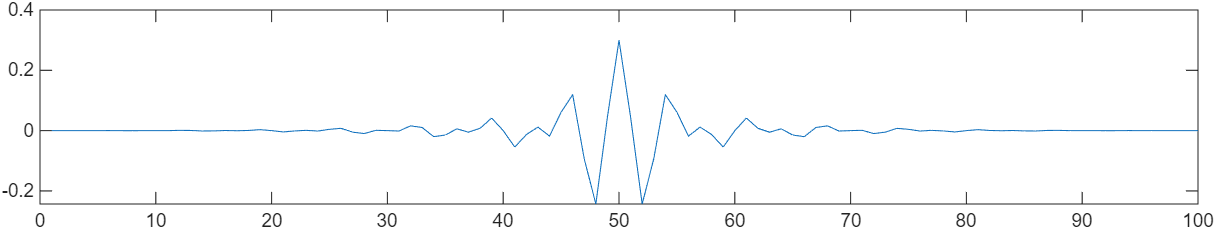
\includegraphics[width=0.82\textwidth]{fig_4_fpf_tempo.png}
\caption{Resposta ao impulso do filtro passa-faixa (FPF).}
\label{fig:4_fpf_t}
\end{figure}

\begin{figure}[H]
\centering
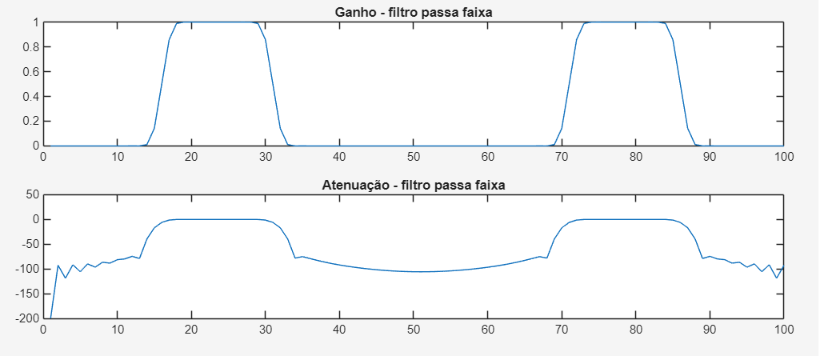
\includegraphics[width=0.82\textwidth]{fig_4_fpf_freq.png}
\caption{Resposta em frequ\^encia do FPF: banda de passagem entre $0{,}15$ e $0{,}30$.}
\label{fig:4_fpf_f}
\end{figure}

\begin{figure}[H]
\centering
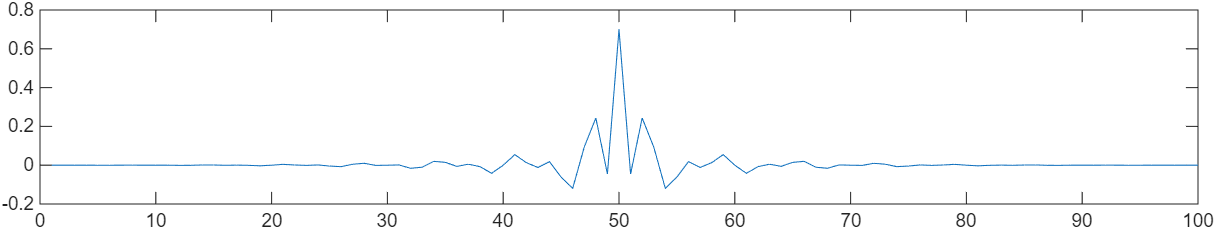
\includegraphics[width=0.82\textwidth]{fig_4_fcf_tempo.png}
\caption{Resposta ao impulso do filtro corta-faixa (FCF).}
\label{fig:4_fcf_t}
\end{figure}

\begin{figure}[H]
\centering
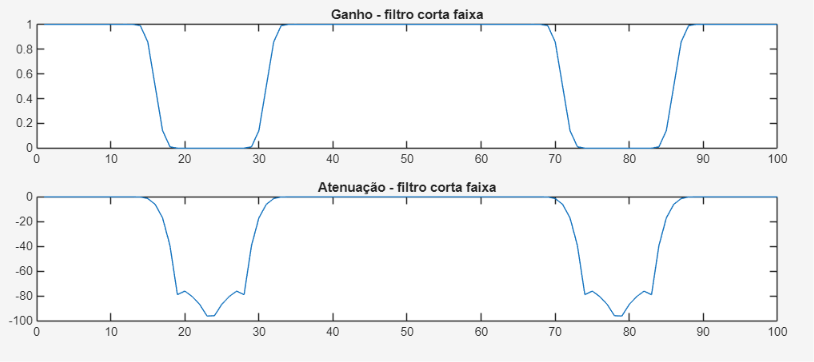
\includegraphics[width=0.82\textwidth]{fig_4_fcf_freq.png}
\caption{Resposta em frequ\^encia do FCF: rejei\c{c}\~ao da faixa entre $0{,}15$ e $0{,}30$.}
\label{fig:4_fcf_f}
\end{figure}

As respostas confirmam o projeto: o FPF apresenta banda de passagem bem definida
entre $0{,}15$ e $0{,}30$ (com os pontos de $-6$~dB exatamente nas frequ\^encias de
corte) e forte atenua\c{c}\~ao fora dela; o FCF, ao contr\'ario, mant\'em ganho
unit\'ario nas duas bandas externas e abre um entalhe (\textit{notch}) profundo na
faixa central. Como as bandas de transi\c{c}\~ao das janelas de Blackman ($M=100$)
n\~ao se sobrep\~oem entre $0{,}15$ e $0{,}30$, a soma do FCF resulta em um entalhe
limpo, sem o ac\'umulo de ganho que ocorreria com cortes mais pr\'oximos.

% ==================== QUESTAO 5 ====================
\section*{Quest\~ao 5: Filtragem do sinal $x(n)$}

\subsection*{5.a) Gera\c{c}\~ao do sinal}

O sinal de teste, com $1000$ amostras, \'e a soma de tr\^es sen\'oides:
%
\begin{equation}
x(n) = \sin\!\Big(\tfrac{\pi\,100\,n}{1000}\Big)
      + \sin\!\Big(\tfrac{\pi\,500\,n}{1000}\Big)
      + \sin\!\Big(\tfrac{\pi\,800\,n}{1000}\Big).
\end{equation}
%
Reescrevendo $\sin(\pi\,k\,n/1000) = \sin(2\pi\,(k/2)\,n/1000)$, as frequ\^encias
normalizadas (ciclos por amostra) s\~ao $0{,}05$, $0{,}25$ e $0{,}40$, que numa FFT
de $1000$ pontos correspondem aos \textit{bins} $50$, $250$ e $400$ (com os espelhos
em $600$, $750$ e $950$).

\begin{lstlisting}[caption={Gera\c{c}\~ao do sinal $x(n)$.}]
n = 1:1000;
x = sin(pi*100*n/1000) + sin(pi*500*n/1000) + sin(pi*800*n/1000);
figure(1); plot(n, x);  title('x(n) no tempo');
figure(2); plot(abs(fft(x)));  title('Espectro de x(n)');
\end{lstlisting}

\begin{figure}[H]
\centering
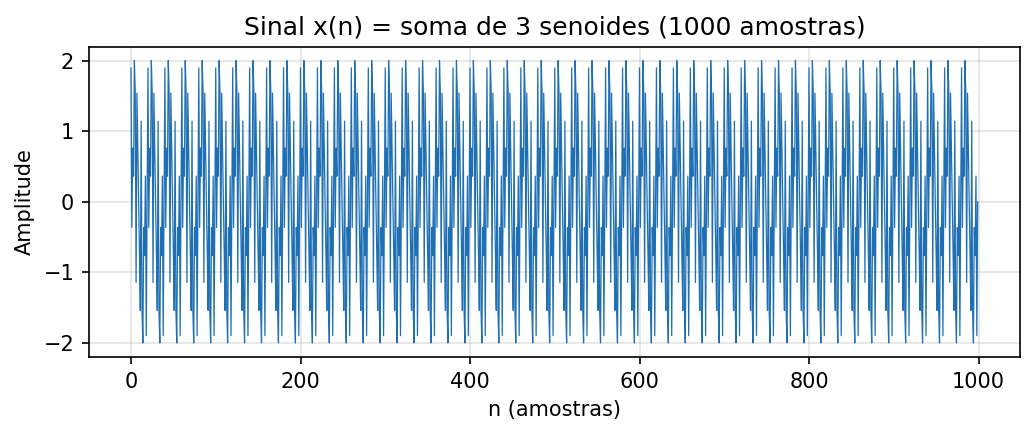
\includegraphics[width=0.82\textwidth]{fig_5_x_tempo.png}
\caption{Sinal $x(n)$ no dom\'inio do tempo (1000 amostras).}
\label{fig:5_xt}
\end{figure}

\begin{figure}[H]
\centering
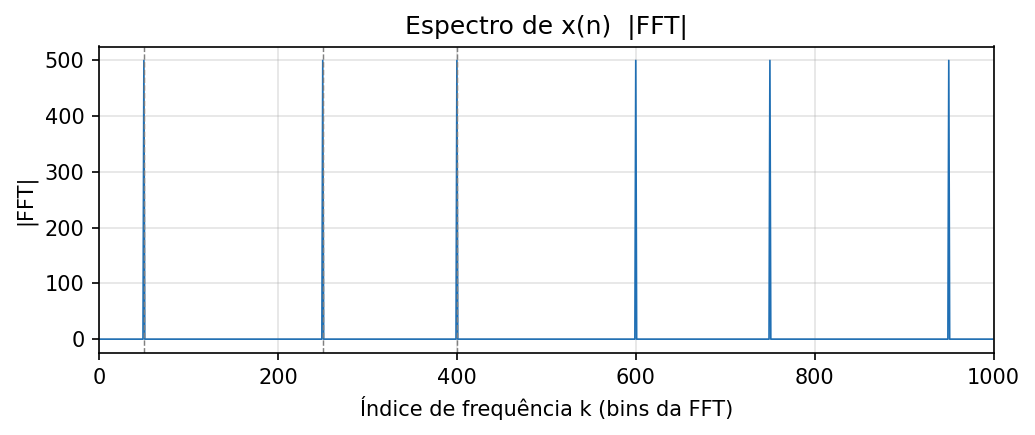
\includegraphics[width=0.82\textwidth]{fig_5_x_freq.png}
\caption{Espectro $|\text{FFT}|$ de $x(n)$: raias em $50$, $250$ e $400$ (e espelhos).}
\label{fig:5_xf}
\end{figure}

\subsection*{5.b) Filtragem com os quatro filtros}

O sinal foi filtrado, por convolu\c{c}\~ao, com os quatro filtros dos itens 2 a 4
(passa-baixas e passa-altas com $FC=0{,}15$, al\'em do passa-faixa e do
corta-faixa). Os resultados, no tempo e na frequ\^encia, s\~ao mostrados a seguir.

\begin{lstlisting}[caption={Filtragem do sinal pelos quatro filtros.}]
yPB = conv(x, FPB);   yPA = conv(x, FPA);
yPF = conv(x, FPF);   yCF = conv(x, FCF);
figure; plot(yPB);            figure; plot(abs(fft(yPB)));
% ... idem para yPA, yPF e yCF
\end{lstlisting}

\begin{figure}[H]
\centering
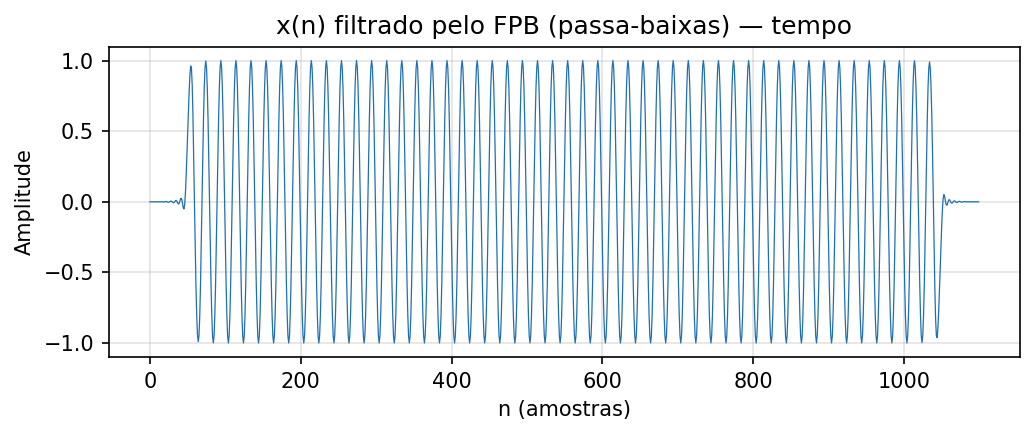
\includegraphics[width=0.49\textwidth]{fig_5_pb_tempo.png}\hfill
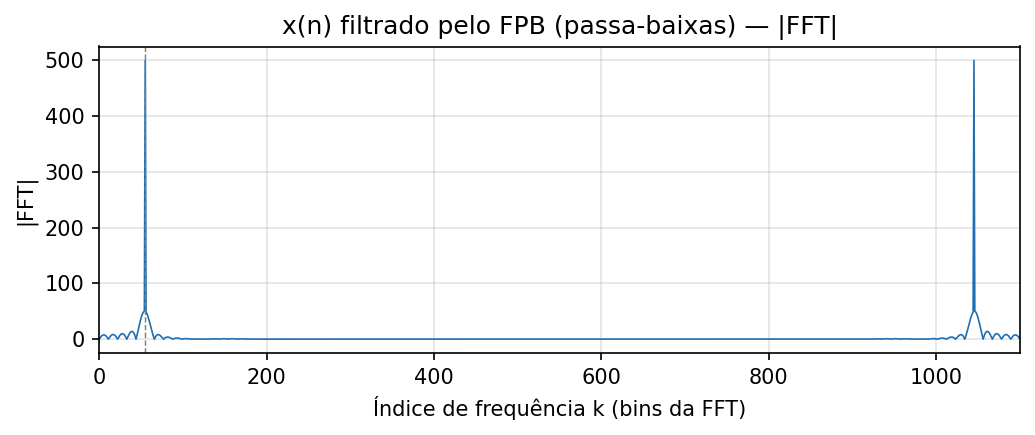
\includegraphics[width=0.49\textwidth]{fig_5_pb_freq.png}
\caption{$x(n)$ filtrado pelo FPB (passa-baixas): sobra apenas a raia de $0{,}05$.}
\label{fig:5_pb}
\end{figure}

\begin{figure}[H]
\centering
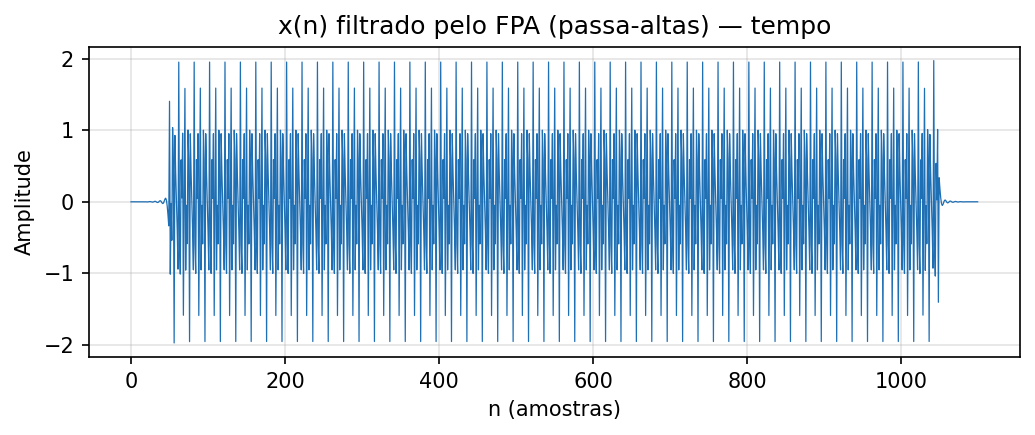
\includegraphics[width=0.49\textwidth]{fig_5_pa_tempo.png}\hfill
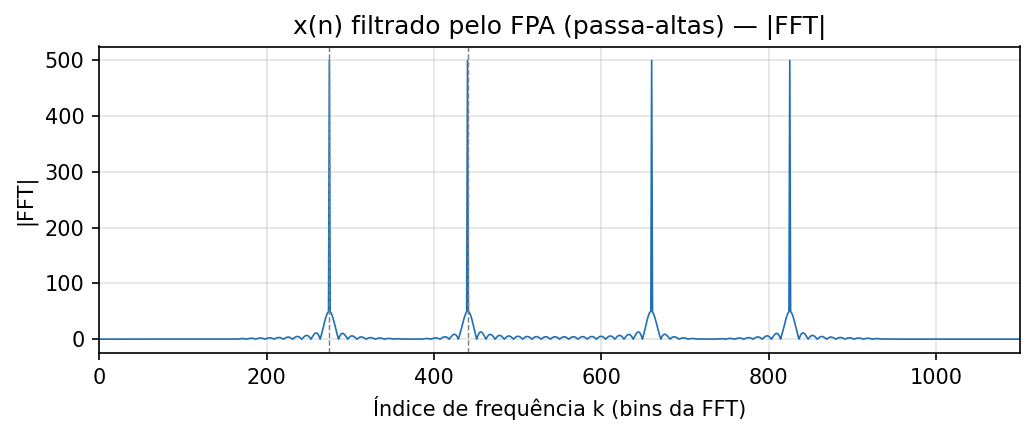
\includegraphics[width=0.49\textwidth]{fig_5_pa_freq.png}
\caption{$x(n)$ filtrado pelo FPA (passa-altas): sobram as raias de $0{,}25$ e $0{,}40$.}
\label{fig:5_pa}
\end{figure}

\begin{figure}[H]
\centering
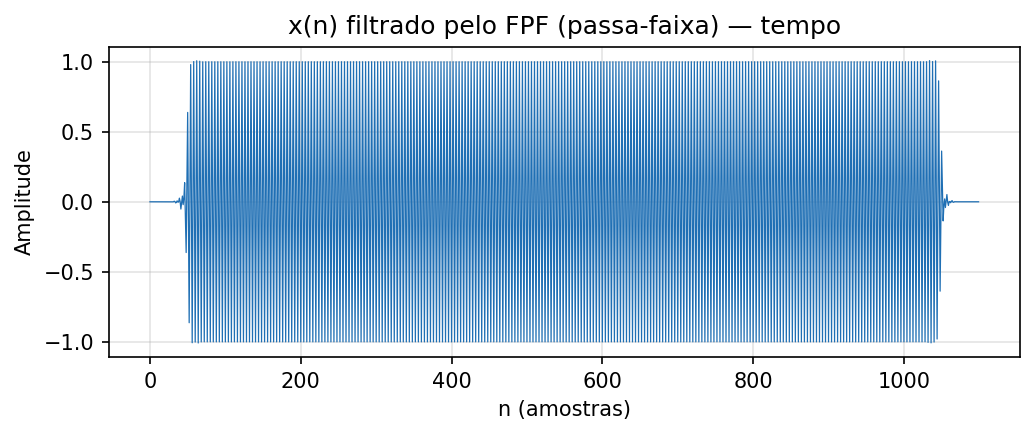
\includegraphics[width=0.49\textwidth]{fig_5_pf_tempo.png}\hfill
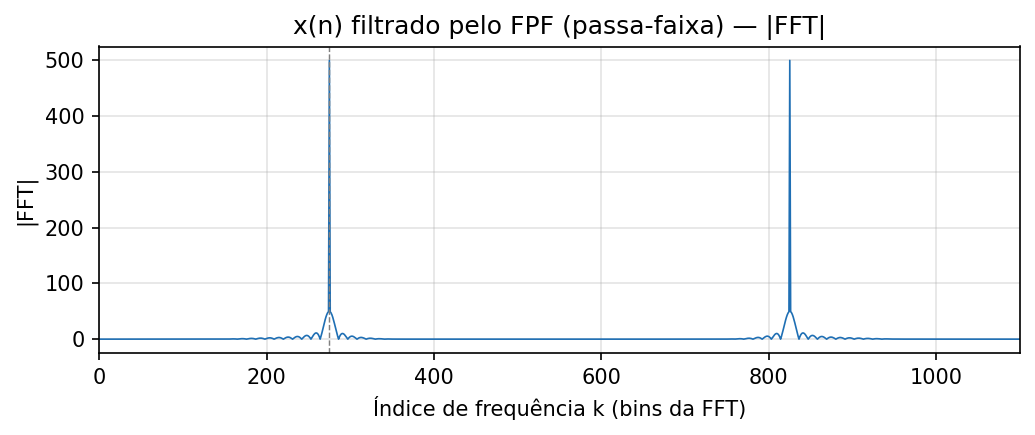
\includegraphics[width=0.49\textwidth]{fig_5_pf_freq.png}
\caption{$x(n)$ filtrado pelo FPF (passa-faixa): sobra apenas a raia de $0{,}25$.}
\label{fig:5_pf}
\end{figure}

\begin{figure}[H]
\centering
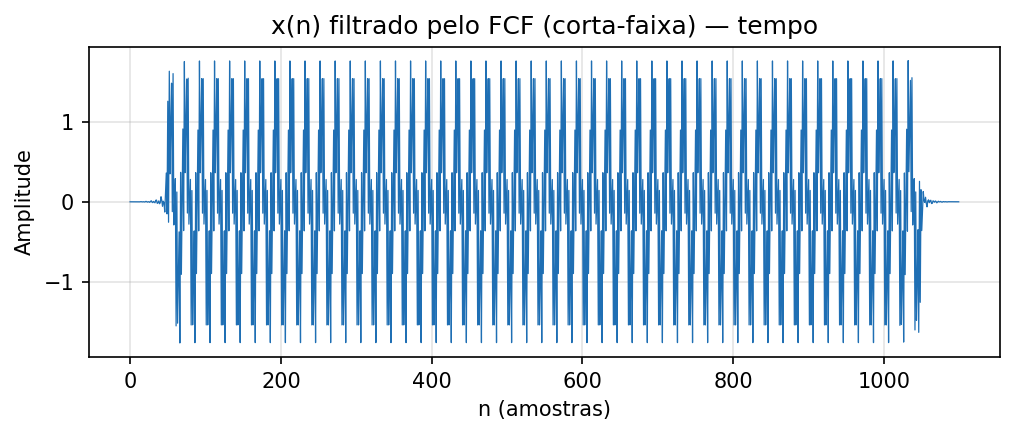
\includegraphics[width=0.49\textwidth]{fig_5_cf_tempo.png}\hfill
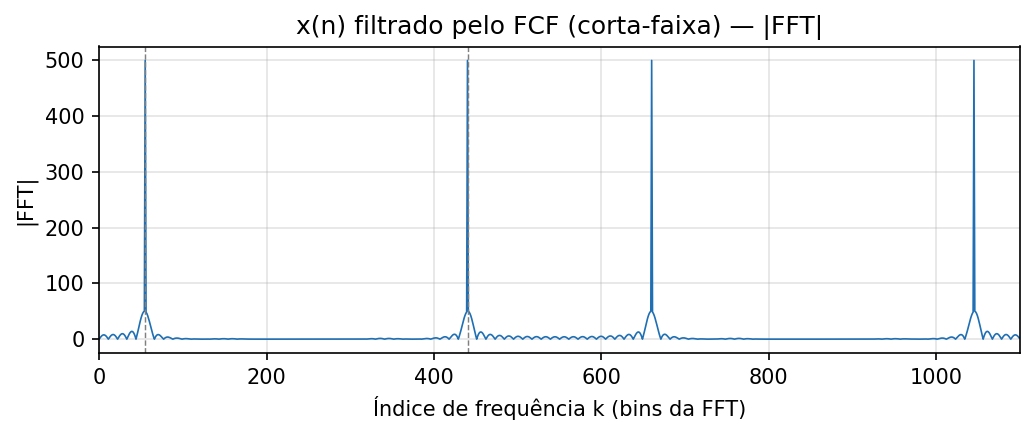
\includegraphics[width=0.49\textwidth]{fig_5_cf_freq.png}
\caption{$x(n)$ filtrado pelo FCF (corta-faixa): sobram $0{,}05$ e $0{,}40$;
a raia de $0{,}25$ \'e rejeitada.}
\label{fig:5_cf}
\end{figure}

Cada filtro atua exatamente como projetado: o FPB preserva s\'o a componente de
baixa frequ\^encia; o FPA, apenas as duas mais altas; o FPF isola a componente
intermedi\'aria ($0{,}25$); e o FCF elimina justamente essa componente central,
preservando as demais. Note-se que as raias aparecem deslocadas em rela\c{c}\~ao
\`as do sinal original (por exemplo, a de $0{,}05$ migra do \textit{bin} $50$ para o
$55$), fen\^omeno analisado na Quest\~ao~6.

% ==================== QUESTAO 6 ====================
\section*{Quest\~ao 6: Deslocamento das raias ap\'os a filtragem}

A convolu\c{c}\~ao de um sinal de $N = 1000$ amostras com um filtro de $M+1 = 101$
coeficientes produz um sinal mais longo, de $N + M = 1100$ amostras. Como a FFT
distribui os seus \textit{bins} ao longo de todo o comprimento do registro, uma
componente que ocupava o \textit{bin} $k$ na FFT de $1000$ pontos passa a ocupar o
\textit{bin}
%
\begin{equation}
k' = k \cdot \frac{N + M}{N},
\end{equation}
%
na FFT de $1100$ pontos. Isso explica as posi\c{c}\~oes observadas:

\begin{table}[H]
\centering
\begin{tabular}{cccc}
\toprule
Raia & \textit{bin} original ($N{=}1000$) & \textit{bin} previsto $k'$ & \textit{bin} medido \\
\midrule
$0{,}05$ & $50$  & $55$  & $55$  \\
$0{,}25$ & $250$ & $275$ & $275$ \\
$0{,}40$ & $400$ & $440$ & $440$ \\
\bottomrule
\end{tabular}
\caption{Deslocamento das raias: previs\~ao $k' = k\,(N{+}M)/N$ \textit{vs.} medi\c{c}\~ao.}
\end{table}

\'E importante notar que \textbf{n\~ao houve mudan\c{c}a real de frequ\^encia}. A
frequ\^encia normalizada de cada componente, $f = k/N$, permanece a mesma:
$50/1000 = 55/1100 = 0{,}05$; $250/1000 = 275/1100 = 0{,}25$; e
$400/1000 = 440/1100 = 0{,}40$. O que mudou foi apenas a \textbf{escala de
\textit{bins} da FFT}, pois o sinal filtrado ficou mais longo. Em outras palavras,
o deslocamento das raias \'e um efeito do aumento do n\'umero de amostras provocado
pela convolu\c{c}\~ao, e n\~ao uma altera\c{c}\~ao do conte\'udo espectral do sinal.

% ==================== QUESTAO 7 ====================
\section*{Quest\~ao 7: Separa\c{c}\~ao da imagem h\'ibrida (Marilyn / Einstein)}

A imagem h\'ibrida do arquivo \texttt{ImagemHibrida1s2025.mat} (matriz de
$497 \times 408$) combina a foto de Marilyn Monroe, formada por \textbf{baixas
frequ\^encias} espaciais, com a de Einstein, formada por \textbf{altas
frequ\^encias}. Tratando cada linha da matriz como um vetor unidimensional, um
filtro passa-baixas separa a Marilyn e um passa-altas separa o Einstein.

\begin{lstlisting}[caption={Filtragem da imagem h\'ibrida linha a linha.}]
load('ImagemHibrida1s2025.mat');
IH = Imagem_hibrida;
figure(1); imshow(IH, []);          % imagem original

fc = 0.05;  M = 60;                  % parametros escolhidos
WindowSincPB = FWSPB(M, fc);
WindowSincPA = FWSPA(M, fc);

[lin, col] = size(IH);
ini = M/2;                           % descarta o transiente da convolucao
for i = 1:lin
    mb = conv(IH(i,:), WindowSincPB);
    ma = conv(IH(i,:), WindowSincPA);
    hibrida_PB(i,:) = mb(ini+1 : ini+col);   % regiao central ('same')
    hibrida_PA(i,:) = ma(ini+1 : ini+col);
end
figure(2); imshow(hibrida_PB, []);   % Marilyn (baixas frequencias)
figure(3); imshow(hibrida_PA, []);   % Einstein (altas frequencias)
\end{lstlisting}

\paragraph{Como chegamos aos par\^ametros.} Por serem filtros complementares,
adotou-se a \textbf{mesma frequ\^encia de corte} $fc$ para o passa-baixas e o
passa-altas, de modo que juntos eles particionem o espectro exatamente em $fc$.
Para escolher $fc$ fizemos uma varredura ($fc \in \{0{,}03,\ 0{,}05,\ 0{,}10\}$),
mostrada na Figura~\ref{fig:7_escolha}:

\begin{itemize}
\item com $fc = 0{,}10$ o corte \'e alto demais -- o passa-baixas come\c{c}a a
``vazar'' tra\c{c}os do Einstein para dentro da Marilyn e, simultaneamente, o
passa-altas perde quase todo o conte\'udo do Einstein;
\item com $fc = 0{,}03$ o Einstein sai bem n\'itido, mas a Marilyn perde parte da
sua riqueza tonal (fica excessivamente borrada);
\item com $fc = 0{,}05$ obt\^em-se o melhor compromisso: a Marilyn sai limpa, sem
res\'iduos do Einstein, e o Einstein \'e recuperado com bom contraste. Esse valor
corresponde, na pr\'atica, \`a frequ\^encia de cruzamento usada na constru\c{c}\~ao
da imagem h\'ibrida.
\end{itemize}

A ordem $M = 60$ foi escolhida por estreitar a banda de transi\c{c}\~ao (melhorando
a separa\c{c}\~ao em torno de $fc$) sem que o n\'ucleo se torne grande frente \`a
largura da imagem ($408$ colunas). Por fim, como a convolu\c{c}\~ao alonga cada
linha, descartamos as $M/2$ amostras de transiente de cada borda (regi\~ao central,
equivalente ao modo \textit{same}) e usamos um realce de contraste de $1$ a $99\%$
para a visualiza\c{c}\~ao, j\'a que a sa\'ida do passa-altas tem m\'edia nula e
amplitude pequena.

\begin{figure}[H]
\centering
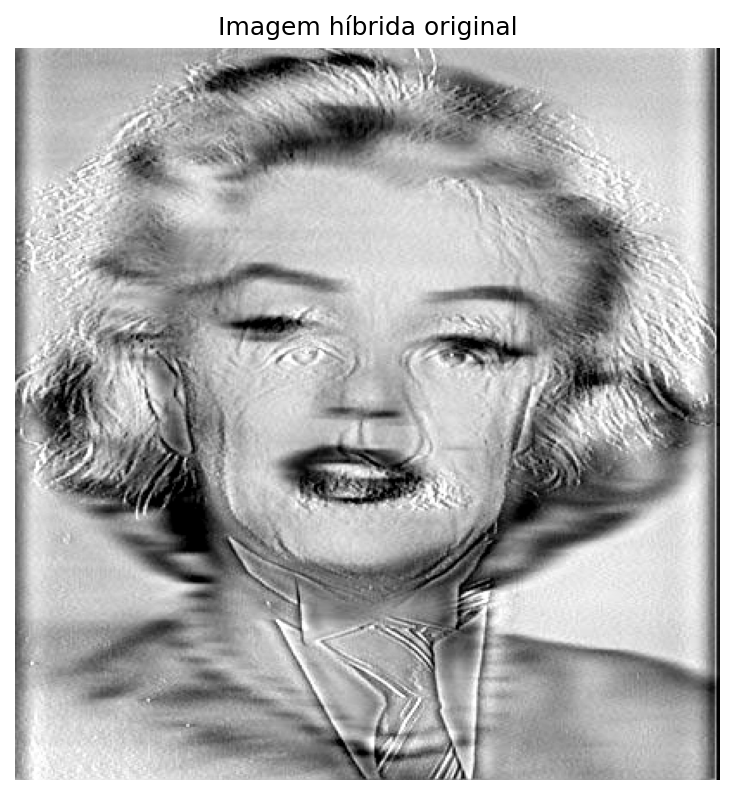
\includegraphics[width=0.45\textwidth]{fig_7_original.png}
\caption{Imagem h\'ibrida original.}
\label{fig:7_orig}
\end{figure}

\begin{figure}[H]
\centering
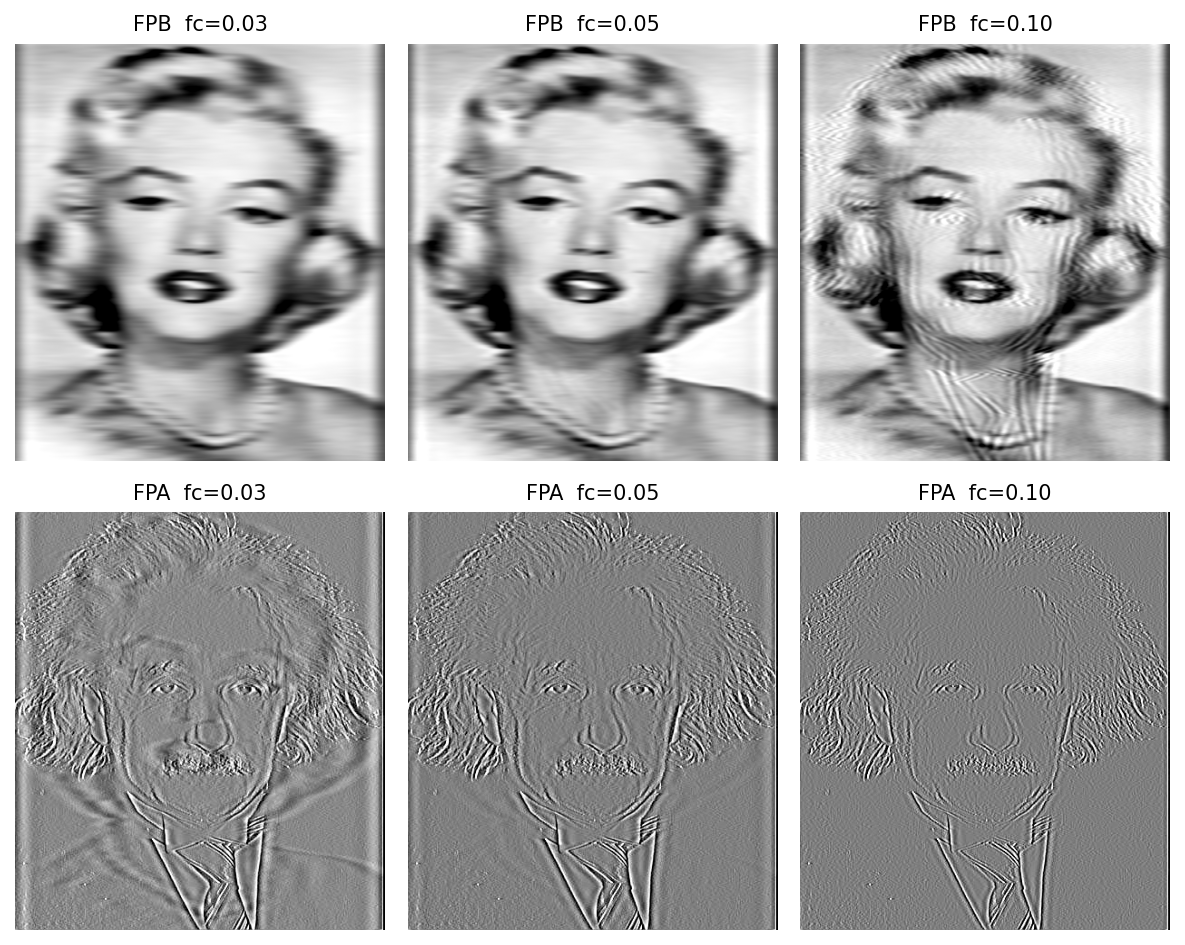
\includegraphics[width=0.88\textwidth]{fig_7_escolha.png}
\caption{Varredura de $fc$ para a escolha do par\^ametro. Linha superior: passa-baixas
(Marilyn); linha inferior: passa-altas (Einstein). Em $fc=0{,}05$ obt\^em-se a melhor
separa\c{c}\~ao.}
\label{fig:7_escolha}
\end{figure}

\begin{figure}[H]
\centering
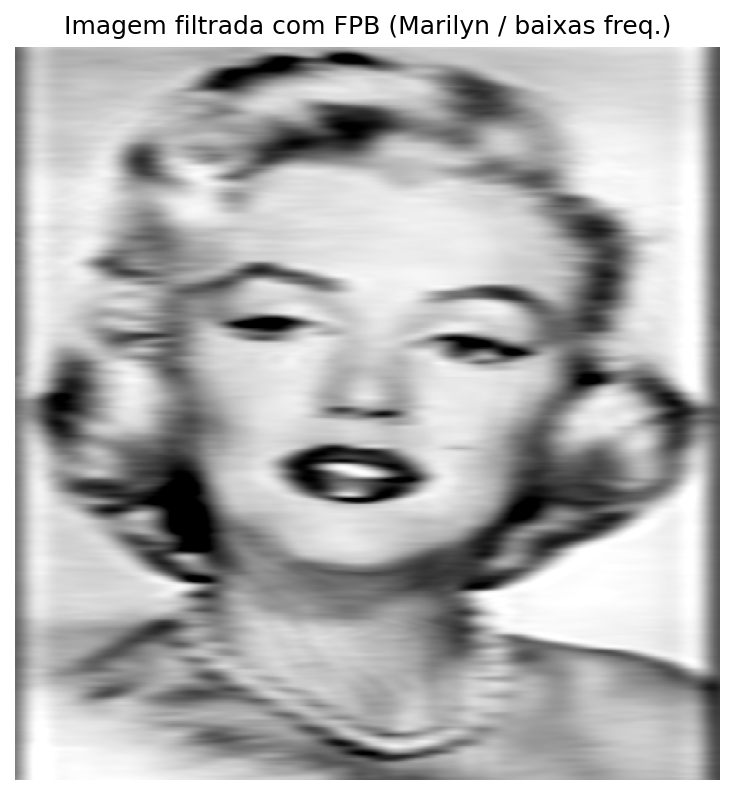
\includegraphics[width=0.45\textwidth]{fig_7_marilyn.png}\hfill
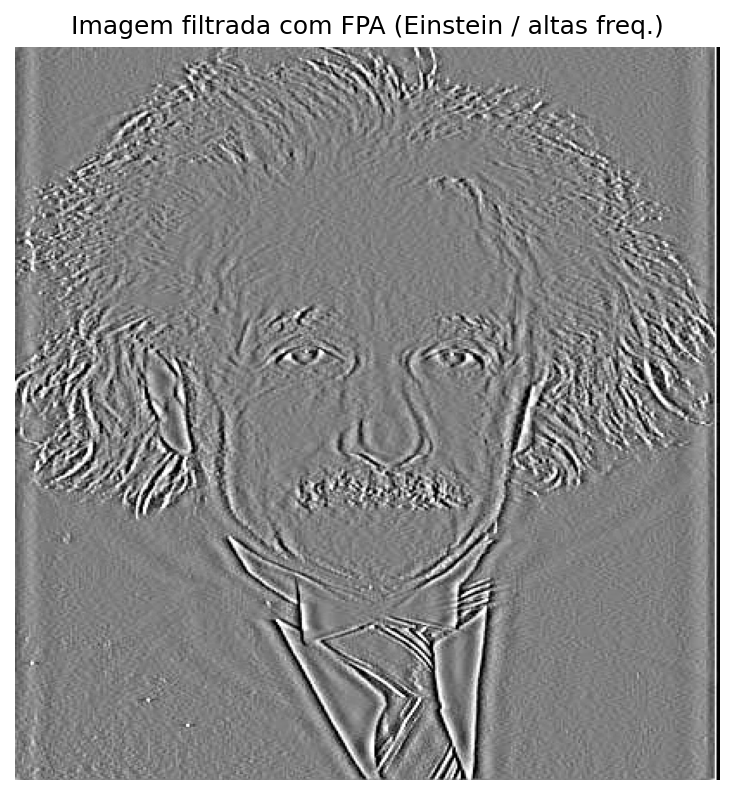
\includegraphics[width=0.45\textwidth]{fig_7_einstein.png}
\caption{Resultado final ($fc = 0{,}05$, $M = 60$). \`A esquerda, a imagem filtrada
pelo FPB (Marilyn, baixas frequ\^encias); \`a direita, pelo FPA (Einstein, altas
frequ\^encias).}
\label{fig:7_result}
\end{figure}

O passa-baixas recupera a Marilyn de forma suave e n\'itida, enquanto o passa-altas
revela o Einstein em forma de bordas realçadas sobre um fundo cinza (efeito de
\textit{emboss}), t\'ipico de um filtro de altas frequ\^encias, que remove o
componente cont\'inuo da imagem.

% ==================== CONCLUSAO ====================
\section*{Conclus\~ao}

A pr\'atica permitiu projetar e analisar filtros FIR pelo m\'etodo
\textit{Window-sinc}. Implementou-se o passa-baixas com a janela de Blackman e,
comparando com a vers\~ao sem janela, verificou-se que o janelamento elimina o
\textit{ripple} de Gibbs e melhora muito a atenua\c{c}\~ao da banda de
rejei\c{c}\~ao (de cerca de $-30$ dB para menos de $-90$ dB), ao custo de uma
transi\c{c}\~ao um pouco mais larga.

Em seguida, obteve-se o passa-altas por invers\~ao espectral e, a partir dos
filtros b\'asicos, constru\'iram-se o passa-faixa (cascata/convolu\c{c}\~ao) e o
corta-faixa (paralelo/soma), ambos com $100$ pontos. A filtragem do sinal de tr\^es
sen\'oides confirmou a seletividade de cada filtro e evidenciou que o discreto
deslocamento das raias decorre apenas do aumento do n\'umero de amostras causado pela
convolu\c{c}\~ao -- a frequ\^encia normalizada $k/N$ permanece inalterada.

Por fim, o m\'etodo foi aplicado ao processamento da imagem h\'ibrida, separando-se
Marilyn (baixas frequ\^encias) e Einstein (altas frequ\^encias) por filtragem das
linhas, com a escolha de $fc$ e $M$ justificada por uma varredura de par\^ametros. O
trabalho consolidou os conceitos de janelamento, invers\~ao espectral, associa\c{c}\~ao
de filtros e convolu\c{c}\~ao, fundamentais em An\'alise de Sistemas Lineares.

\end{document}
